\section{Git Basics}

\begin{frame}{Installing git}

    sudo apt install git

    pacman -S git

    yum install git

    \begin{description}
        \item{For Linux:} http://git-scm.com/download/linux
        \item{For Mac:} http://git-scm.com/download/mac
        \item{For Windows:} http://git-scm.com/download/win
    \end{description}

\end{frame}

\begin{frame}[fragile]{How it works}
    \begin{minipage}{\textwidth}
        \begin{figure}
            \centering
            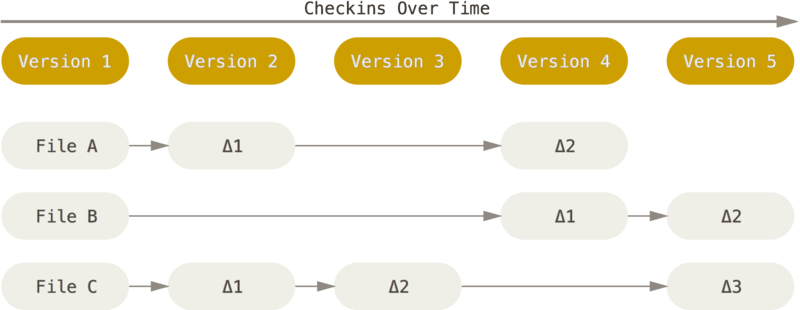
\includegraphics[width=0.8\textwidth]{img/filebased.png}
            \caption{storing changes to a base file}
        \end{figure}
    \end{minipage}
    \begin{minipage}{\textwidth}
        \begin{figure}
            \centering
            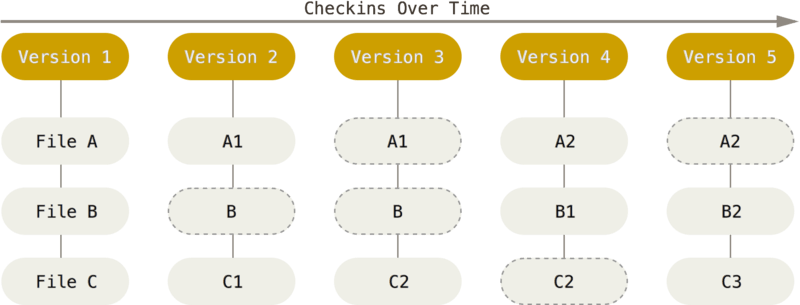
\includegraphics[width=0.8\textwidth]{img/snapshotbased.png}
            \caption{storing snapshots over time}
        \end{figure}
    \end{minipage}
\end{frame}

\begin{frame}{How it works}

    \begin{itemize}
        \item most operations are local
        \item entire history is locally available
    \end{itemize}

    integrety
    everything is check-summed before and then referrenced to by that checksum
    sha1 40 charcter string hex decode
    git stores everything by hash value of its contents instead of its filename

    git only adds data

    three states
    - commited
    - modified
    - staged
    - (untracked)

\end{frame}

\begin{frame}{What is a git repository?}

    \begin{figure}
        \centering
        \includegraphics[width=0.9\textwidth]{img/three_states.png}
    \end{figure}
\end{frame}

\begin{frame}{Basic Workflow}
    \begin{enumerate}
        \item modify files in your working directory
        \item stage the files, adding snapshots fo them to your staging area
        \item commit, stores the snapshot in the staging area permanently in
            your git directory.
    \end{enumerate}
\end{frame}

\defverbatim\setusername{%
    \scriptsize
    \verb+git config --global user.name "Max Mustermann"+
    \newline
}
\defverbatim\setusermail{%
    \scriptsize
    \verb+git config --global user.mail "max.mustermann@example.org"+
    \newline
}

\begin{frame}{Configure git}

    Place where the git configuration can live:
    % TODO: take a table for that
    \begin{itemize}
            \item \textit{/etc/gitconfig} system wide configuration
                \textit{--system}
            \item \textit{~/.gitconfig} or \textit{~/.config/gitconfig}  user wide configuration \textit{--global}
            \item \textit{.git/config} repository specific configuration
    \end{itemize}

\end{frame}

\begin{frame}[fragile]{Setup Your Environment}
    Three essentail configuration values you should have set.
    \begin{itemize}
        \item Your name
        \item Your email address
        \item Your editor
    \end{itemize}
    \begin{lstlisting}
git config --global user.name "Max Mustermann"
git config --global user.mail "max.m@example.org"
git config --global core.editor vim
    \end{lstlisting}
\end{frame}

\begin{frame}[fragile]{git config}
    \emph{Show your configuration}
    \begin{lstlisting}
        git config --list
    \end{lstlisting}

    \emph{Example configurations:}
    \begin{description}
        \item[aliases] \hfill \\
            \begin{lstlisting}
git config alias.st=git status
            \end{lstlisting}
        \item[highlighting] \hfill \\
            \begin{lstlisting}
git config --global color.ui=always
            \end{lstlisting}
    \end{description}

\end{frame}

\begin{frame}[fragile]{Lets Start\ldots}
    Start from scratch\ldots
    \begin{lstlisting}
mkdir my_new_project; cd my_new_project
git init
    \end{lstlisting}
    or\ldots getting local copy of repository that already exist.\\
    \begin{lstlisting}
git clone https://github.com/blastmaster/ta-git_intro.git
    \end{lstlisting}
\end{frame}

\begin{frame}[fragile]{Clone}
    \emph{When you want to checkout out a git repsoitory use \textit{clone}}
    \begin{lstlisting}
git clone https://github.com/blastmaster/ta-git_intro.git
git clone -b branchname git_url
    \end{lstlisting}
\end{frame}

\begin{frame}{Recording Changes}
    \emph{Each file in your working directory can be in one of two states:
        tracked or untracked.}

    \begin{figure}
        \centering
            \includegraphics[width=\textwidth]{img/file_lifecycle.png}
    \end{figure}

\end{frame}

\begin{frame}[fragile]{Checking the Status}
    % TODO: bild was verschiedene stati zeigt
    \begin{lstlisting}
        git status
    \end{lstlisting}
    \begin{lstlisting}
        git status -s
    \end{lstlisting}

\end{frame}

\begin{frame}[fragile]{Ignoring Files}
    \emph{Ignore files that follow a specific pattern with a \textit{.gitignore} file}

    \textit{.gitignore} rules:
    \begin{itemize}
        \item Black lines or lines starting with \# are ignored.
        \item Standard glob pattern work.
        \item You can start patterns with a forward slash (/) to avoid recusivity.
        \item You can negate a pattern by starting it with an exclamation point (!).
    \end{itemize}

    %TODO: github maintains a large amount of .gitignore files
    %link https://github.com/github/gitignore

\end{frame}

\begin{frame}[fragile]
    \frametitle{What is a git repository?}
    \begin{figure}[b]
        \centering
        \begin{tikzpicture}
            \tikzstyle{state} = [ draw,
                node distance = 1.4em,
                drop shadow = {opacity=0.15},
                font = \fontfamily{lmtt}\selectfont\small,
                shape = rectangle,
                %rounded corners = .5em,
                minimum width = 7em,
                minimum height = 2em,
                text opacity = 0.75,
                semithick ]
            \tikzstyle{whatis} = [
                node distance = 1.4em,
                left,
                font = \fontfamily{lmtt}\selectfont\tiny]
            \node[state] (remote) {remote};
            \node[state] (repository) [below=of remote] {Local Repository};
            \node[state] (index) [below=of repository] {Staging Area};
            \node[state] (stash) [below=of index] {Stash};
            \node[state] (tree)  [below=of stash] {Working Directory};

            \node[whatis, left] at (remote.west) {Repository on the internet or network.};
            \node[whatis, left] at (repository.west) {Local repository that contains complete history.};
            \node[whatis, left] at (index.west) {Snapshot of the working tree for next commit.};
            \node[whatis, left] at (stash.west) {A place to hide modification if you need a clean workspace.};
            \node[whatis, left] at (tree.west) {The direcotries and files on your filesystem.};
        \end{tikzpicture}
    \end{figure}
\end{frame}

\begin{frame}
    \frametitle{Staging files}
    \begin{figure}[b]
        \centering
        \begin{tikzpicture}
            \tikzstyle{state} = [ draw,
                node distance = 1.4em,
                drop shadow = {opacity=0.15},
                font = \fontfamily{lmtt}\selectfont\small,
                shape = rectangle,
                rounded corners = .5em,
                minimum width = 7em,
                minimum height = 2em,
                text opacity = 0.75,
                semithick ]
            \tikzstyle{whatis} = [
                node distance = 1.4em,
                font = \fontfamily{lmtt}\selectfont\tiny]
            \node[state] (index) {Staging Area};
            \node[state] (tree)  [below=of index] {Working Directory}
                edge [->, out=0, in=0] node[whatis, right] {git add <filename>} (index)
                edge [<-, out=180, in=180] node[whatis, left] {git reset HEAD <filename>} (index);
        \end{tikzpicture}
    \end{figure}
\end{frame}

\begin{frame}
    \frametitle{Stashing}
    \begin{figure}[b]
        \centering
        \begin{tikzpicture}
            \tikzstyle{state} = [ draw,
                node distance = 1.4em,
                drop shadow = {opacity=0.15},
                font = \fontfamily{lmtt}\selectfont\small,
                shape = rectangle,
                rounded corners = .5em,
                minimum width = 7em,
                minimum height = 2em,
                text opacity = 0.75,
                semithick ]
            \tikzstyle{whatis} = [
                node distance = 1.4em,
                font = \fontfamily{lmtt}\selectfont\tiny]
            \node[state] (stash) [below=of index] {Stash};
            \node[state] (tree)  [below=of stash] {Working Directory}
                edge [->, out=0, in=0] node [whatis, right] {git stash} (stash)
                edge [<-, out=180, in=180] node [whatis, left] {git apply} (stash);
        \end{tikzpicture}
    \end{figure}
\end{frame}


\begin{frame}
    \frametitle{commiting changes}
    \begin{figure}[b]
        \centering
        \begin{tikzpicture}
            \tikzstyle{state} = [ draw,
                node distance = 1.4em,
                drop shadow = {opacity=0.15},
                font = \fontfamily{lmtt}\selectfont\small,
                shape = rectangle,
                rounded corners = .5em,
                minimum width = 7em,
                minimum height = 2em,
                text opacity = 0.75,
                semithick ]
            \tikzstyle{whatis} = [
                node distance = 1.4em,
                font = \fontfamily{lmtt}\selectfont\tiny]
            \node[state] (repository)  {local repository};
            \node[state] (index) [below=of repository] {Staging Area}
                edge [->, out=0, in=0] node [whatis, right] {git commit} (repository);
            \node[state] (tree)  [below=of stash] {Working Directory}
                edge [<-, out=180, in=180] node [whatis, left] {git checkout <commitid>} (repository)
                edge [->, out=0, in=0] node[whatis, right] {git add <filename>} (index);
        \end{tikzpicture}
    \end{figure}
\end{frame}


\begin{frame}
    \frametitle{remote}
    \begin{figure}[b]
        \centering
        \begin{tikzpicture}
            \tikzstyle{state} = [ draw,
                node distance = 1.4em,
                drop shadow = {opacity=0.15},
                font = \fontfamily{lmtt}\selectfont\small,
                shape = rectangle,
                rounded corners = .5em,
                minimum width = 7em,
                minimum height = 2em,
                text opacity = 0.75,
            semithick ]
            \tikzstyle{whatis} = [
                node distance = 1.4em,
                font = \fontfamily{lmtt}\selectfont\tiny]
                \node[state] (remote) {remote: origin};
                \node[state] (working) [below=of remote] {local repository}
                edge [<-, in=0, out=0]  node[whatis, right] {git pull origin master} (remote)
                edge [->, in=180, out=180] node[whatis, left] {git push origin master} (remote);
        \end{tikzpicture}
        \includegraphics[width=\textwidth]{img/show_remote.png}
    \end{figure}
\end{frame}


\defverbatim\myadd{%
    \scriptsize
    \verb+git remote add github git@github.com:username/repo.git+
    \newline
}

\begin{frame}[fragile]
    \frametitle{adding a remote}
    \myadd
    \begin{figure}
        \centering
        \begin{tikzpicture}
            \tikzstyle{state} = [ draw,
                node distance = 1.4em,
                drop shadow = {opacity=0.15},
                font = \fontfamily{lmtt}\selectfont\small,
                shape = rectangle,
                rounded corners = .5em,
                minimum width = 7em,
                minimum height = 2em,
                text opacity = 0.75,
            semithick ]
            \tikzstyle{whatis} = [
                node distance = 2.4em,
                font = \fontfamily{lmtt}\selectfont\tiny]
                \node[state] (remote) {remote: origin};
                \node[state] (remote2) [right=of remote] {remote: github};
                \node[state] (working) [below=of remote, xshift=1.25cm] {local copy}
                edge [<->, in=180, out=180] node[whatis, left, align=center] {
                    git pull origin master \\
                git push origin master} (remote)
                edge [<->, in=0, out=0] node[whatis, right, align=center] {git pull github master \\
                git push github master} (remote2);
        \end{tikzpicture}
    \end{figure}
\end{frame}

\defverbatim\mytag{%
    \scriptsize
    \verb+git tag -a v0.1 A+
    \newline
}

\begin{frame}[fragile]{Tags}
    Two types of tags
    - lightweight tags (much like a branch that dosen't change, its just a pointer to
    a specific commit.)
    - annotated tags (full stored objects in the git database)
\end{frame}

\begin{frame}
    \frametitle{Tags}
    Tags are like bookmarks on commits.
    \begin{figure}[b]
        \centering
        \begin{tikzpicture}
            \gitDAG[grow right sep = 2em]
            {
                A -- B -- C
            };
            \gitbranch
            {master}
            {above=of C}
            {C}
            \gitHEAD
            {above=of master}
            {master}
        \end{tikzpicture}
        \caption{lets create a tag for commit A}
    \end{figure}
\end{frame}

\begin{frame}[fragile]{Annotated Tags}
    \emph{Creating an annotated tag by specify -a.}
    % -m for the tagging message
    \begin{description}
        \item[create tag] git tag -a <commitid>
        \item[delete tag] git tag -d <tagname>
        \item[filter tag] git tag -l <pattern>
        \item[sign tag] git tag -s <tagname>
    \end{description}
    \textbf{Showing a tag:}
    \begin{lstlisting}
        git show v1.4
    \end{lstlisting}
\end{frame}

\begin{frame}[fragile]{Sharing Tags}
    \textbf{You need to explicitly transfer tags to remote.}
    \begin{lstlisting}
        git push origin <tagname>
    \end{lstlisting}
    or:
    \begin{lstlisting}
        git push origin --tags
    \end{lstlisting}
    \textbf{Checking out Tags:}
    \begin{lstlisting}
        git checkout -b <branchname> <tagname>
    \end{lstlisting}
\end{frame}

\begin{frame}[fragile]{Tags}
    \mytag
    \begin{figure}[b]
        \centering
        \begin{tikzpicture}
            \gitDAG[grow right sep = 2em]
            {
                A -- B -- C
            };
            \gitbranch {master}
            {above=of C}
            {C}
            \gittag
            [v0p1]
            {v0.1}
            {above=of A}
            {A}
            \gitHEAD
            {above=of master}
            {master}
        \end{tikzpicture}
        \caption{our brand new tag!}
    \end{figure}
\end{frame}

\begin{frame}
    \frametitle{Branching}
    \begin{figure}[b]
        \centering
        \begin{tikzpicture}
            \gitDAG[grow right sep = 2em]
            {
                A -- B -- C
            };
            \gitbranch {master}
            {above=of C}
            {C}
            \gittag
            [v0p1]
            {v0.1}
            {above=of A}
            {A}
            \gitHEAD
            {above=of master}
            {master}
        \end{tikzpicture}
        \caption{lets create a new branch}
    \end{figure}
\end{frame}

\begin{frame}
    \frametitle{Branch Syntax}
    \begin{description}
        \item[create new branch] \hfill \\
            \begin{itemize}
                \item git branch <branchname>
                \item git checkout -b <branchname>
            \end{itemize}
        \item[delete branch] \hfill \\
            \begin{itemize}
                \item git branch -d <branchname>
            \end{itemize}
    \end{description}
\end{frame}

\begin{frame}
    \frametitle{Branching}
    \begin{figure}[b]
        \centering
        \begin{tikzpicture}
            \gitDAG[grow right sep = 2em]
            {
                A -- B -- {
                    C,
                    D -- E,
                }

            };
            \gitbranch {master}
            {above=of C}
            {C}
            \gittag
            [v0p1]
            {v0.1}
            {above=of A}
            {A}
            \gitbranch
            {feature X}
            {above=of E}
            {E}
            \gitHEAD
            {above=of master}
            {master}
        \end{tikzpicture}
        \caption{lets create a new branch}
    \end{figure}
\end{frame}

\begin{frame}
    \frametitle{Rebasing}
    \begin{figure}
        \centering
        \begin{tikzpicture}
            \gitDAG[grow right sep = 2em]
            {
                A -- B -- {
                    C,
                    D -- E,
                }
            };
            \gittag
            [v0p1]
            {v0.1}
            {above=of A}
            {A}
            \gitremotebranch
            [origmaster]
            {origin/master}
            {above=of C}
            {C}
            \gitbranch
            {master}
            {above=of E}
            {E}
            \gitHEAD
            {above=of master}
            {master}
        \end{tikzpicture}
    \end{figure}
\end{frame}

\begin{frame}
    \frametitle{Rebasing}
    \begin{figure}
        \centering
        \begin{tikzpicture}
            \gitDAG[grow right sep = 2em] {
                A -- B -- {
                    C -- D' -- E',
                    {[nodes=unreachable] D -- E},
                }
            };
            \gittag
            [v0p1]
            {v0.1}
            {above=of A}
            {A}
            \gitremotebranch
            [origmaster]
            {origin/master}
            {above=of C}
            {C}
            \gitbranch
            {master}
            {above=of E'}
            {E'}
            \gitHEAD
            {above=of master}
            {master}
        \end{tikzpicture}
    \end{figure}
\end{frame}

% demonstrate merging of two branches
\begin{frame}
    \frametitle{merging}
    \begin{figure}[b]
        \centering
        \begin{tikzpicture}
            \gitDAG[grow right sep = 2em]
            {
                A -- B -- {
                    C,
                    D -- E,
                }
            };
            \gitbranch
            {master}
            {above=of C}
            {C}
            \gitbranch
            {feature X}
            {above=of E}
            {E}
            \gitHEAD
            {above=of feature X}
            {feature X}
        \end{tikzpicture}
        \caption{Before\ldots}
    \end{figure}
\end{frame}

\begin{frame}
    \frametitle{merging}
    \begin{figure}[b]
        \centering
        \begin{tikzpicture}
            \gitDAG[grow right sep = 2em]
            {
                A -- B --{
                C,
                    {D -- E},
                } -- E'
            };
            \gitbranch
            {master}
            {above=of E'}
            {E'}
            \gitbranch
            {feature X}
            {below=of E}
            {E}
            \gitHEAD
            {above=of master}
            {master}
        \end{tikzpicture}
        \caption{after: \texttt{git merge feature X}}
    \end{figure}
\end{frame}

\begin{frame}[fragile]{Follow the Changes}
    \begin{description}
        \item[what:] git diff [-\,-staged]
        % if you prefer a graphical or external diff viewing program instead.
        % there is `git difftool` for you
        % `git difftool --tool-help` to see whats available
        \item[when:] git log
        \item[who:] git blame
    \end{description}
\end{frame}

\begin{frame}[fragile]{Working with the log}
    \centering
    \adjustbox{max height=\dimexpr\textheight-5.5cm\relax,
               max width=\textwidth}{
    \begin{tabular}{ll}
        \textbf{Option} & \textbf{Description} \\ \hline
        \textit{-(n)} & Show only the last $n$ commits\\ \hline
        \textit{-\,-since, -\,-after} & Limit the commits to those made after the specified date.\\ \hline
        \textit{-\,-unitl, -\,-before} & Limit the commit to those made before the specified date.\\ \hline
        \textit{-\,-author} & Only show commits in which the author entry matches specified string.\\ \hline
        \textit{-\,-committer} & Only show commits in which the committer entry matches the specified string.\\ \hline
        \textit{-\,-grep} & Only show commits with a commit message containing the string.\\ \hline
        \textit{-S}  & Only show commits adding or removing code matching the string.\\ \hline
    \end{tabular}
    }
\end{frame}

\begin{frame}[fragile]{Undoing things}

    \textbf{Unstating a Staged File:}
    \begin{lstlisting}
        git restet HEAD <file>
    \end{lstlisting}
    \textbf{Unmodifying a Modified File:}
    \begin{lstlisting}
        git checkout -- <file>
    \end{lstlisting}

\end{frame}


\begin{frame}[fragile]{Working with Remotes}
    \textbf{Showing your remotes:}
    \begin{lstlisting}
        git remote -v
    \end{lstlisting}
    \textbf{Showing remote information:}
    \begin{lstlisting}
        git remote show <remote>
    \end{lstlisting}
    \textbf{Rename a remote:}
    \begin{lstlisting}
        git remote rename <oldname> <newname>
    \end{lstlisting}
    \textbf{Remove a remote:}
    \begin{lstlisting}
        git remote rm <remote>
    \end{lstlisting}

\end{frame}


\begin{frame}
    \frametitle{Reference}
    \begin{itemize}
        \item \url{http://www.git-scm.com/docs} % reference
        \item \url{http://www.git-scm.com/book/en/v2} % book
        \item \url{https://sandofsky.com/blog/git-workflow.html} % workflow
        \item \url{http://ndpsoftware.com/git-cheatsheet.html} % cheatcheet
    \end{itemize}
\end{frame}
